\documentclass{article}

\usepackage{graphicx}
\usepackage{subcaption}
\usepackage{amsmath}

\title{AIML426 Project 1 Report}
\date{}

\begin{document}
\maketitle
\section*{Part 1}
\subsection*{Individual Representation}
For this GA the chromosome is represented through a bit vector whose length is the number of possible items to choose from, each element represents a possible item to select for the knapsack. For decoding the chromosome into a solution, for each bit, 1 represents selecting the item while 0 represents not selecting the item.  \par
\noindent Since the order of the items picked up does not matter, the order of items in the chromosome can be the same as the order of items in the weight and values list. This means that the value and weight can be easily obtained by looking at the index of the chosen item in the chromosome in the values and weights lists. The crossover and mutation genetic operators can easily be applied to the chromosome and the solution can be decoded no matter how much the chromosome has changed. \par
\subsubsection*{Individual Generation}
\noindent At first for individual generation a random bit list of range of items length was generated. This worked for the first two datasets, but a problem that was encountered with the third dataset is that it has a large range of items to select, but has a small weight constraint. Thus the majority of individual generated violated the constraint by a lot and the initial population have 0 total fitness and never improve for a long time. \par
\noindent To avoid this the constraint was implemented into the individual generation for the initial population so that all the individuals satisfied the constraint. This was done by starting with a 0 chromosome and setting bits to 1 randomly in the chromosome until the weight constraint has been reached. This will still give a diverse range of individuals while setting the initial population fitness to above 0 and thus having a greater chance of improving the overall population fitness before convergence. \par
\subsection*{Fitness Function}
The fitness of the knapsack solutions is measured in the maximum value of items chosen while also satisfying the maximum weight constraint. The evaluate the maximum value of the knapsack solution, the sum of values of the items selected is calculated. To implement the constraint a penalty variable is introduced, the formula that is used to evaluate when to use the penalty variable for individual of $M$ bits is 
\begin{center} 
$max(0, \sum_{i=1}^{M}v_i - \alpha *max(0,\sum_{i=1}^{M}w_i)-max weight)$. 
\end{center}
So, when the total weight of the solution is greater than the maximum weight, the penalty is applied. A minimum fitness of 0 is set since negative fitness does not work with probabilities.
\subsection*{Termination Criteria}
Two stopping criteria were defined for the GA, the first stopping criteria is a maximum number of generations. For both datasets a maximum generation number of 100 was defined. Another stopping criteria was the convergence check where if the generation population fitness did not change enough for 5 generations, then the GA will stop. As this indicates that the GA will not improve in further generations. \par
\subsection*{Genetic Operators}
\subsubsection*{Crossover}
One-point crossover was used for the crossover genetic operator, since the order of the items selected does not matter, no constraints need to be defined for the split position of the crossover. 
\subsubsection*{Mutation}
Local search mutation was used for the mutation genetic operator. Instead of randomly selecting a bit and flipping the value, the flip position with the largest increase in value is selected. This does increase the computation requirement since instead of O(1) complexity it is now O(M) complexity requiring to now iterate through each possible flip, but also increase chance of improving population each generation and reaching convergence early since mutation will be less likely to produce individuals with bad fitness. 
\subsection*{GA Parameter Values}
%Generation Number and Population Size
\subsubsection*{Number of Generations and Population Size}
To achieve close to the optimal value, different population sizes and generation numbers was tuned for each dataset. For the first and second dataset, population size of 50 and generation number of 100 was set since the dataset is small, thus reaching the optimal value can be quicker. For the third dataset, because of the strict constraint, 100 was set for the population size since there are less individuals that will satisfy the constraint of this dataset. This does mean that running the GA for this dataset is very time consuming so the population size did not increase beyond 100.
%Generations until convergence
\subsubsection*{Iterations Until Convergence}
This was set to 5 so that convergence only occurs when it is obvious that the fitness, measured as the average of the top 5 best individuals, no longer changes each generation. Thus saving computation time with the GA avoiding a large number of iterations with no effect. If set too large, the computation time saved becomes small.
%Selection used
\subsubsection*{Selection Scheme Used}
A fitness-proportional/roulette wheel selection scheme is used for this problem. When implementing the roulette wheel selection, the probability: $\frac{fitness(i)}{pop\_fitness}$ is calculated. A higher probability means a higher chance of being selected either for elitism or for parents. This was chosen since a roulette wheel selection is simple to implement and it encourages selecting high fitness solutions through having a larger probability of being chosen. This is also where the maximum weight constraint is implemented through. 
%Alpha value
\subsubsection*{Alpha/Penalty Coefficient}
The penalty coefficient/alpha variable needs to be tuned to the dataset so it is strong enough to generally ignore solutions that violate constraint when selecting individuals, but small enough to still acknowledge solutions that only slightly violate constraint but have very good value sums. \par
\noindent For the first dataset, an alpha value of 2 was selected since the was a small range of items to select from. \par
\noindent For the second dataset, there was a greater range of items to select from so the alpha value was higher to 3. \par
\noindent For the third dataset, while there was a much greater range of items to select and the weight constraint was very small. Thus the alpha value was set very high to make sure that the best individual does not violate the constraint. \par
%Crossover, Mutation, Elitism rates
\subsubsection*{Crossover, Mutation and Elitism Rates}
For both the first and second dataset, the parameter rates used are: 
\begin{center}
\begin{tabular}{|c|c|}
	\hline
	Elitism Rate: & 0.03 \\
	\hline
	Crossover Rate: & 1.0 \\
	\hline
	Mutation Rate: & 0.3 \\
	\hline
\end{tabular}
\end{center}
For the third dataset, a much higher elitism rate was used to encourage more fit individuals for the next generation since fit individuals means that they do not violate the constraint which is difficult to achieve. The parameter rates used are:
\begin{center}
\begin{tabular}{|c|c|}
	\hline
	Elitism Rate: & 0.1 \\
	\hline
	Crossover Rate: & 1.0 \\
	\hline
	Mutation Rate:	& 0.3 \\
	\hline
\end{tabular}
\end{center}
\subsection*{Results}
%show tables here
\begin{figure}[h]
	\centering
	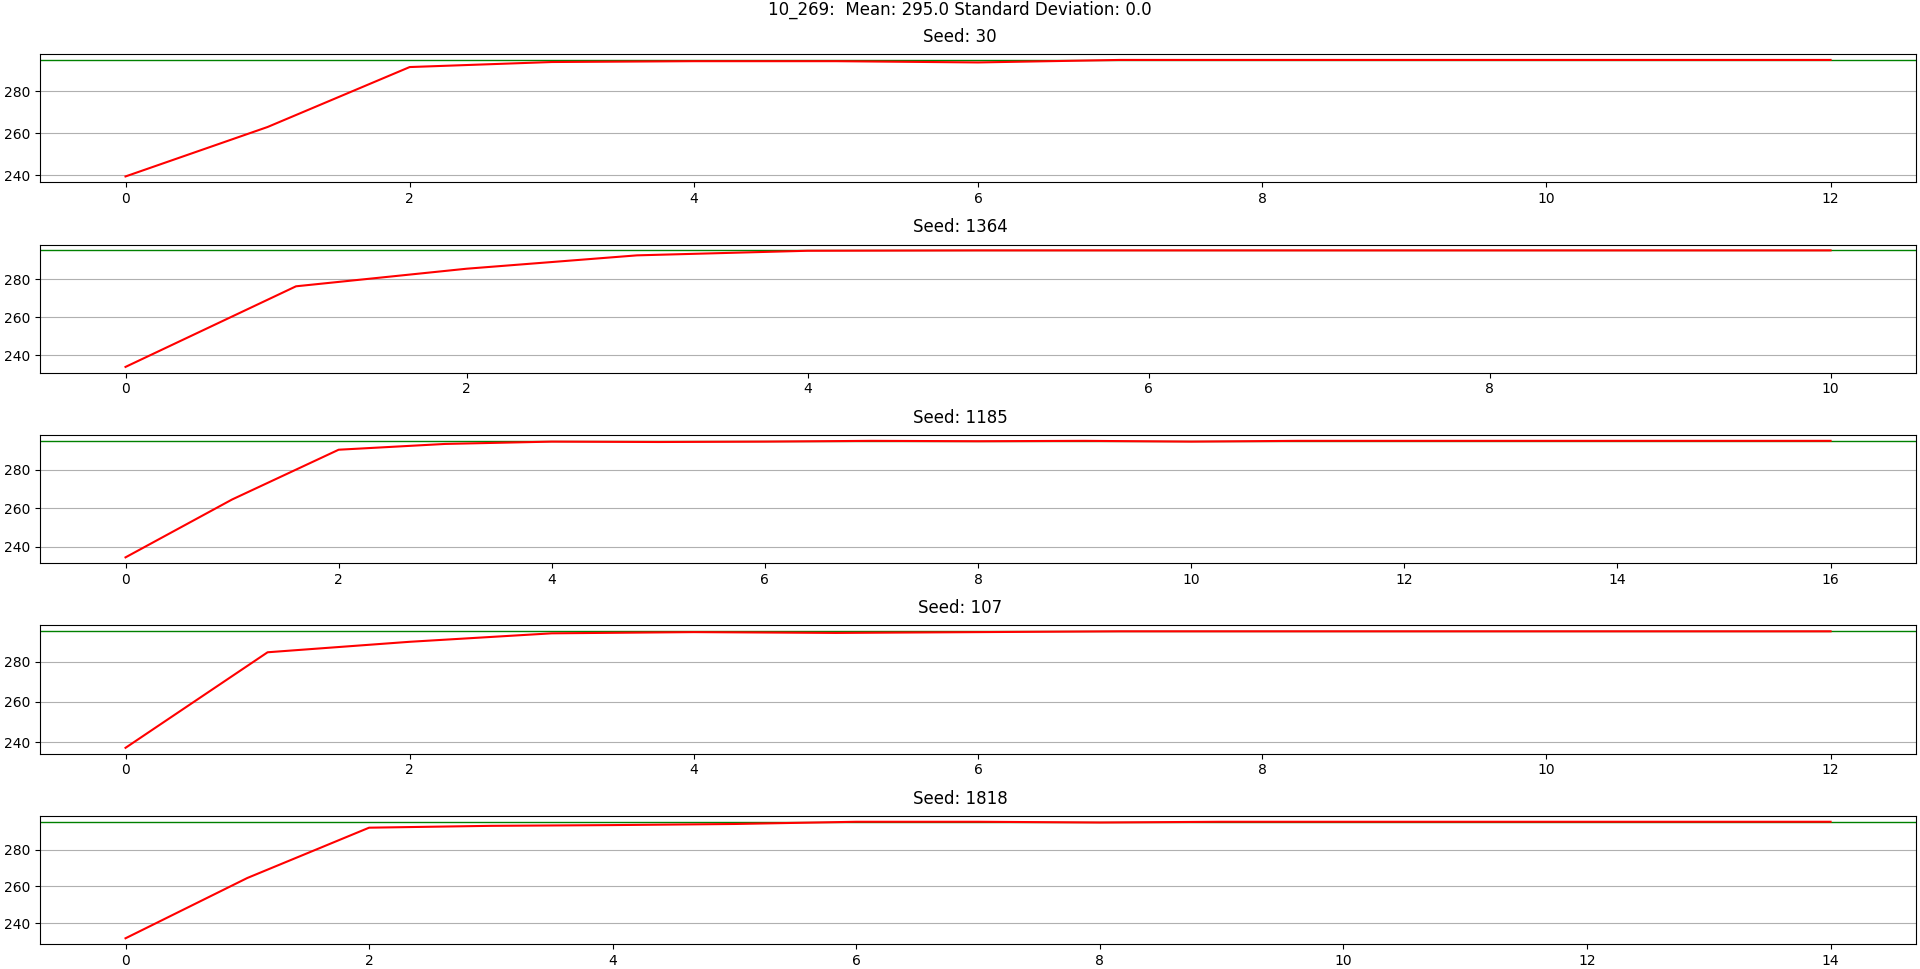
\includegraphics[width=\linewidth]{10_269.png}
	\caption{Convergence curves for dataset 10\_269. Original png image provided as well}
\end{figure}
\begin{figure}[h]
	\centering
	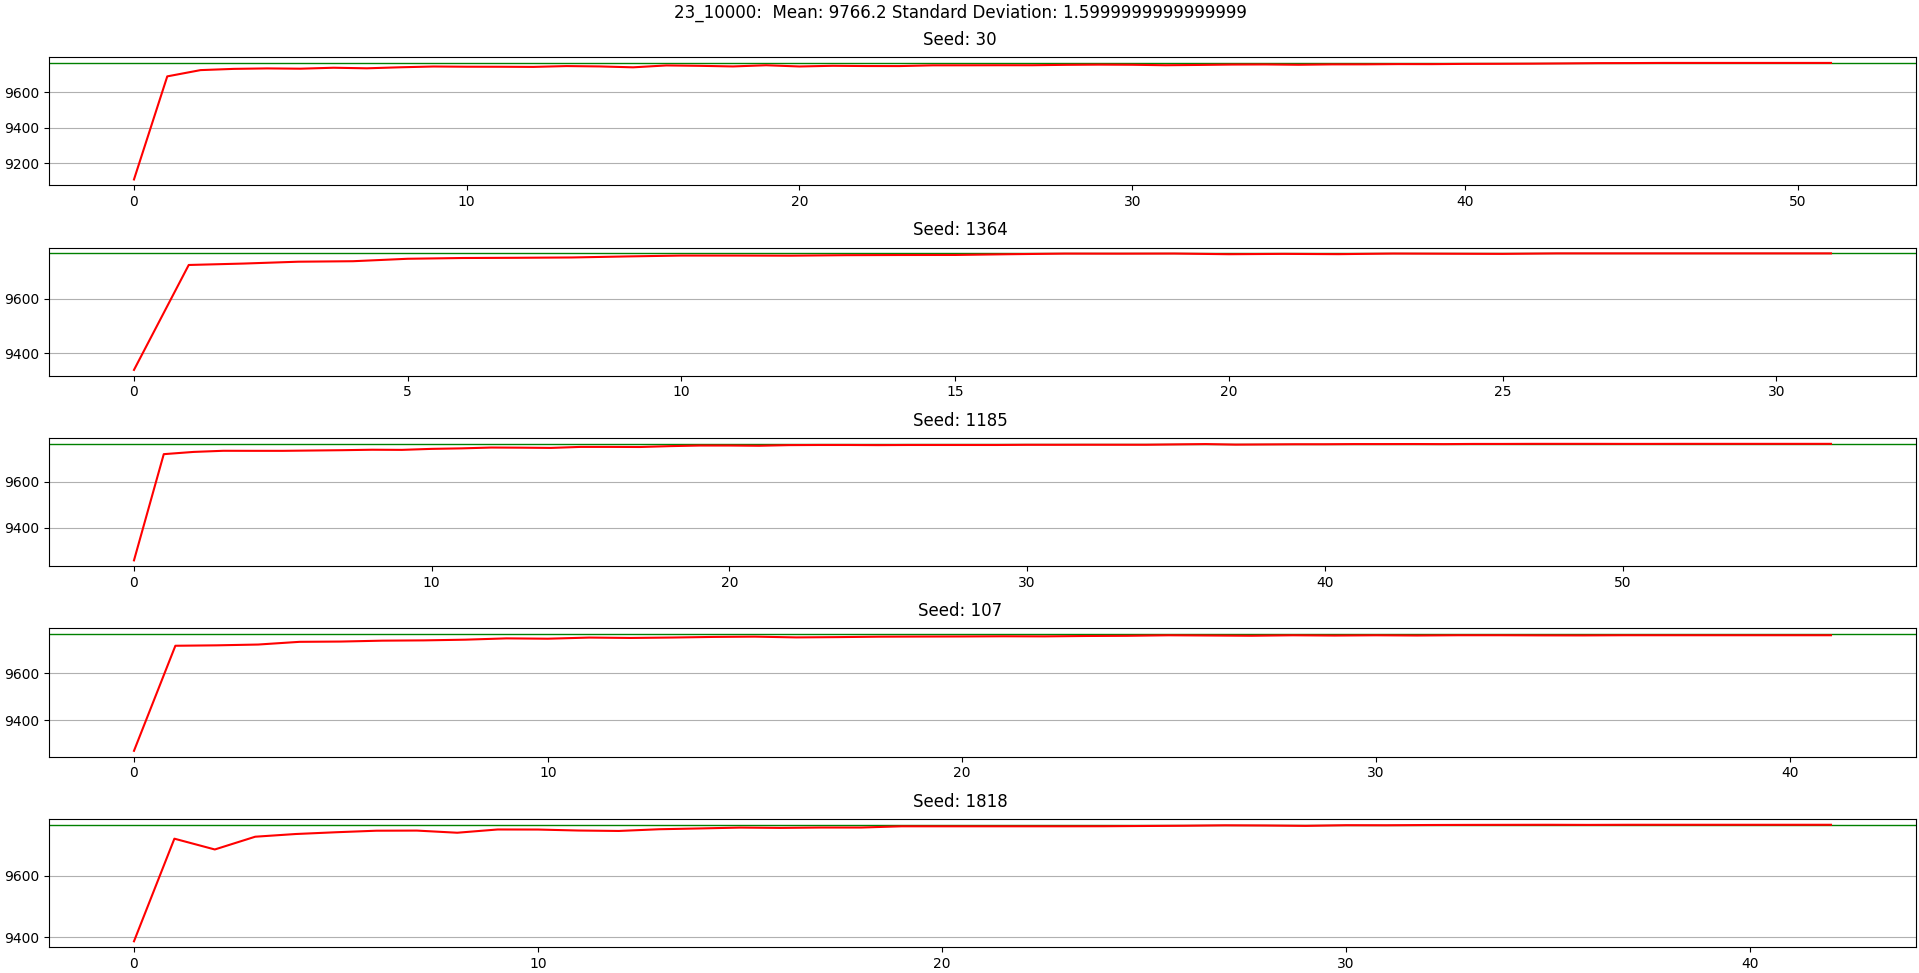
\includegraphics[width=\linewidth]{23_10000.png}
	\caption{Convergence curves for dataset 23\_10000. Original png image provided as well}
\end{figure}
\begin{figure}[h]
	\centering
	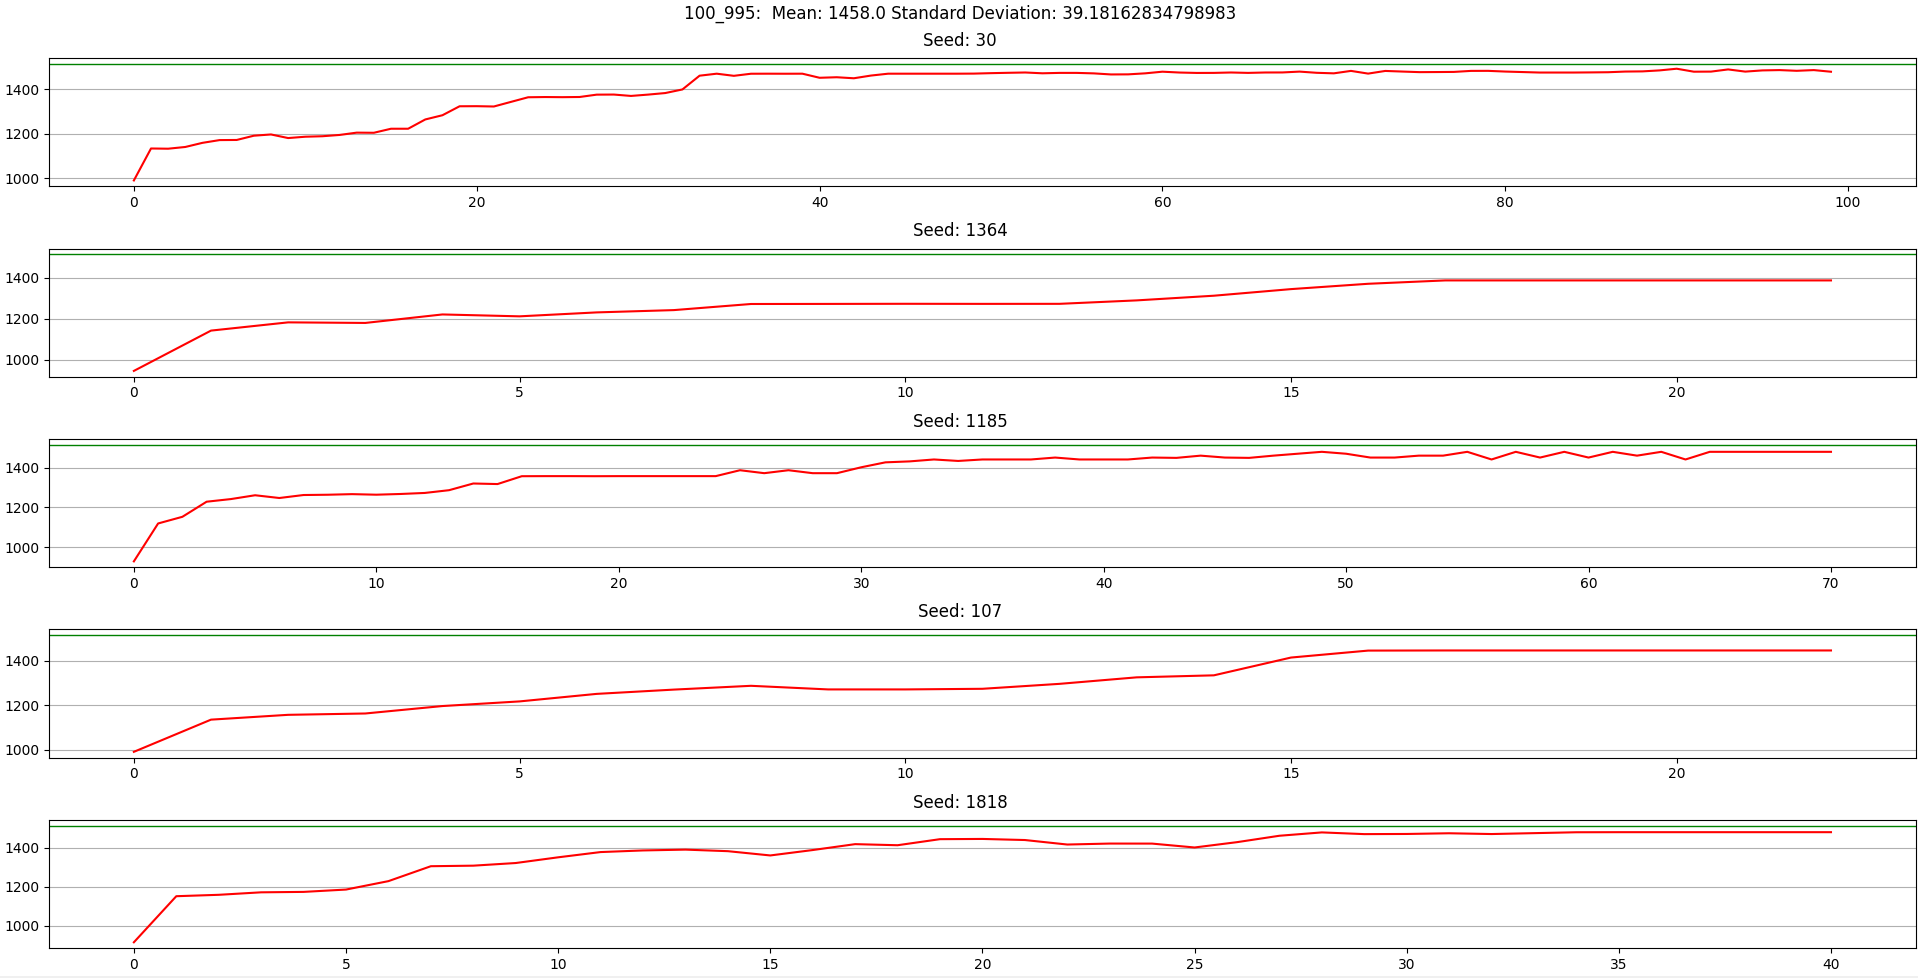
\includegraphics[width=\linewidth]{100_995.png}
	\caption{Convergence curves for dataset 100\_995. Original png image provided as well}
\end{figure}
\clearpage
\subsubsection*{Discussion}
For 10\_269, this dataset converged to the optimal solution in <= 50 generations for all seeds. That means the mean fitness is the same value as the optimal fitness with no deviation. The small range of items to pick from means that exploring all solutions is possible to achieve with GA. This showcases that with the population structure of GA, exploring a large range of solutions can be done within a reasonable number of generations. \par
\noindent For 23\_10000 less generations were needed to reach the optimal solution with all five seeds reaching the optimal value with no deviation. Like in 10\_269 there is a logarithmic relation between the average best fitness of the generation with the number of generations showcasing that this dataset took a while to reach convergence despite being close to the optimal fitness. This could be circumvented by decreasing the mutation rate to prevent minor fitness changes in each generation that stopped convergence. \par
\noindent For 100\_995 none of the seeds reached the optimal solution of 1514 though three of the five seeds were close to the optimal solution. With the mean fitness being noticeably lower than the optimal fitness and with a large standard deviation, this showcases that the seed value has a bigger effect on the final solution compared to the other datasets. Since the weight constraint for this dataset was very small and there are a large range of items to select from, most of all the possible instances violate the constraint. Trying to find the few instances that satisfy the constraint while still trying to achieve a high value sum required finetuning of the parameters until a decent result was produced. Since all the seeds converged before reaching the maximum number of iterations, this showcases a higher rate of mutation was needed, but increasing the mutation rate also increases the likelihood of violating the constraint. The output could be improved with a higher population size, but more computation time would be needed. Several instances of the GA could be run with different seeds with the final output being the best output out of all the individual GA’s best output since different seed values produce variety while also satisfying the constraint. \par
\subsubsection*{Conclusion}
GA is a useful technique for finding optimal or near optimal solutions with it succeeding to finding optimal solutions for small datasets within a reasonable timeframe. The parameters used for the datasets could be worked on more to increase accuracy and performance of the GA to achieve a balance of searching through a large range of solutions without getting stuck in a local optima while still approaching the global optima over time. \par
\noindent GA does struggle with constraints, especially very strict constraints which most solutions violate. Since GAs can easily generate solutions that violate the constraint through reproduction. While implementing the penalty coefficient into the fitness evaluation can help define the constraint into the population, it needs to be balanced to encourage variety and sometimes still struggles to get solutions that are close to the optimal value while not violating the constraint. \par
\section*{Part 2}
\subsection*{Individual Representation}
Feature selection has the same individual representation as the knapsack problem where a bit vector is used to decide if to select the feature(represented as 1) or to ignore the feature(represented as 0). This was chosen because both problems of a very similar problem definition of selecting features/items for the final solution. \par
\subsubsection*{Individual Generation}
For the generation of individuals in the initial population, no constraint is defined for the fitness so the NumPy random number generator is used to generate a random bit vector whose length is equal to the total number of features in each instance in the dataset. \par
\subsection*{Fitness Function}
\subsubsection*{Filter Fitness}
Filter fitness uses information gain where the fitness of the selection subset is determined by the largest amount of information gain. To avoid the bias towards features with a large range of values, symmetric uncertainty was used for the fitness evaluation. Symmetrical uncertainty, compared to information gain ratio, considers not just the range of values in the features(X), but the range of values in the labels(Y) as well. While the range of values in X are much greater than Y in this problem and thus this issue is not as important, this does make the fitness function more flexible for datasets with a large range of class labels. \par
\subsubsection*{Wrapper Fitness}
The wrapper fitness evaluation is determined by the accuracy of the predicted labels output generated by a classifier. This fitness evaluation is run for every individual in the population each generation, so speed is important to consider. Several classifiers were tested for the wrapper fitness, this was done by generating 20 random selected feature subsets and measuring the average accuracy and time taken to evaluate the fitness.  \par
\begin{center}
\begin{tabular}{|c|c|c|}
\hline
Classifier & Speed(seconds) & Accuracy(in \%)\\
\hline
MLP max iter = 1000 & \multicolumn{2}{c|}{wbcd} \\
\hline
& 1.380s & 89.868\% \\
\hline
& \multicolumn{2}{c|}{sonar} \\
\hline
 & 2.464s & 80.595\% \\
\hline
KNN n\_neighbours = 5 & \multicolumn{2}{c|}{wbcd} \\
& 0.0233s & 92.807\% \\
\hline
& \multicolumn{2}{c|}{sonar} \\
\hline
& 0.0223s & 77.857\% \\
\hline
Decision Trees & \multicolumn{2}{c|}{wbcd} \\
& 0.0113s & 92.281\% \\
\hline
& \multicolumn{2}{c|}{sonar} \\
\hline
& 0.0138s & 73.095\% \\
\hline
GaussianNB & \multicolumn{2}{c|}{wbcd} \\
& 0.0101s & 93.289\% \\
\hline
& \multicolumn{2}{c|}{sonar} \\
\hline
& 0.0124s & 69.881\% \\
\hline
\end{tabular}
\end{center}
KNN was chosen since it had the second highest accuracy out of the classifiers explored. Yet it is much faster compared to the MLP classifier. \par
\subsection*{Termination Criteria}
The same termination criteria of max iterations and convergence used for the knapsack problem was used for the feature selection since the two problems are similar. The maximum convergence iterations is set to 5 for both datasets and the maximum number of iterations was defined to be 20 for wbcd and 100 for sonar due to sonar being a larger dataset than wbcd and thus will take more time to evaluate. \par
\subsection*{Genetic Operators}
The genetic operators implemented for knapsack has been reused for this problem because it uses the same individual representation and the feature selection problem aims to maximize the fitness value evaluated by the fitness functions. \par
\subsection*{Discussion}
To measure the time taken by the GAs the Python function time.time() was used to record the time just before the creation of the GA object and just after the evaluation for the final solution of the GA. The time taken for each seed and dataset and the average and standard deviation was calculated. \par
\noindent For measuring the performance of the GA the best individual in the final generation was selected and the MLP classifier was applied to the dataset of selected features. This classifier was chosen since MLP gives the highest accuracy and since this accuracy evaluation is only run a few times the slow time of the MLP classifier does not affect the evaluation time. 
\begin{center}
%Display the table of time and performance 
\begin{tabular}{|c|c|c|}
\hline
Fitness & Average Time(seconds) & Standard Deviation Time(seconds) \\
\hline
FilterGA & \multicolumn{2}{c|}{wbcd} \\
\hline
& 137.505s & 6.170s \\
\hline
& \multicolumn{2}{c|}{sonar} \\
\hline
& 695.327s & 13.814s \\
\hline
WrapperGA & \multicolumn{2}{c|}{wbcd} \\
\hline
& 19.471s & 2.090s \\
\hline
& \multicolumn{2}{c|}{sonar} \\
\hline
& 282.266s & 39.191s \\
\hline
\end{tabular}
\begin{tabular}{|c|c|c|}
\hline
Fitness & Average Performance & Standard Deviation Performance \\
\hline
FilterGA & \multicolumn{2}{c|}{wbcd} \\
\hline
& 91.228\% & 4.114\% \\
\hline
& \multicolumn{2}{c|}{sonar} \\
\hline
& 82.857\% & 4.617\% \\
\hline
WrapperGA & \multicolumn{2}{c|}{wbcd} \\
\hline
& 93.158\% & 0.656\% \\
\hline
& \multicolumn{2}{c|}{sonar} \\
\hline
& 80.952\% & 7.222\% \\
\hline
\end{tabular}
\end{center}
Since the sonar dataset has twice as many features compared to the wbcd dataset and more than twice as many instances, more time was taken to evaluate the final feature subset. The filterGA took around 3 times as long to evaluate the final solution compared to the wrapperGA. Thus, the time advantage that the filter fitness usually has, was not applied to this problem. The reason why the filterGA is slower is because of the implementation of the filter fitness evaluation. Unlike the wrapperGA where the classifier was called from a library where it would be optimized, the filter fitness was implemented without using any libraries and thus is very unoptimized. There is also the structure of the datasets, since the filterGA works with discrete features and the features in the datasets are continuous. When the features are discretized, there are no duplicate features and thus the probabilities calculated for each feature were the same. Which could lead to lack of quickly emphasizing certain features through the generations. \par
\noindent The average performance for wrapperGA is similar to the performance of the filterGA, with the filterGA excelling for the sonar dataset. The worse performance by the WrapperGA could have happened due to the KNN classifier used. KNN had good time but only decent accuracy, if the MLP classifier was used then the accuracy of the wrapperGA could be greater than the filterGA but with the time taken to evaluate being greater as well. \par
\subsection*{Conclusion}
For the datasets used, the wrapperGA is the better option due to the use of continuous features in the dataset. If the datasets were much bigger and thus is more time-consuming for the classifiers or if you need the fitness to be independent from the classifier, then the filter fitness would be a better option. \par
\noindent Comparing the filterGA and the wrapperGA on discrete datasets could lead to different results where the filterGA excels due to it being designed for discrete features. \par
\section*{Part 3}
\subsection*{Individual Representation}
Each individual needs to keep track of classification performance and ratio of selected features. The bit vector is used again for this problem where the classification performance is determined by using a wrapper classifier on the features subset and the ratio of selected features is determined by $\frac{\text{Number of 1s in bit vector}}{\text{Total length of bit vector}}$.
\subsubsection*{Individual Generation}
For individual generation, since there are no constraints it uses the same generation as used in Part 2 of generating a random bit value for each element in the vector. 
\subsection*{Fitness Function}
The fitness function is defined by two objectives: classification performance and the feature ratio. The problem’s focus is to maximize the classification performance, which is the same as minimizing the error rate, and minimize the selected feature ratio. Thus, the fitness function is defined as a tuple of (classification, -ratio). 
\subsection*{Genetic Operators}
The same single point split crossover operator that is used in the previous two problems is used for this problem. The mutation operator used here is flip bit mutation but since this problem uses the mutFlipBit operator from the Python library DEAP, the local search feature implemented in the previous two problems is not used here.  \par
\noindent The datasets in the problem use these parameters for the GA: 
\begin{center}
\begin{tabular}{|c|c|c|}
\hline
& vehicle & clean1 \\
\hline
Population Size & 60 & 160 \\
\hline
Generation Size & 80 & 250 \\
\hline
Crossover Rate & 1.0 & 1.0 \\
\hline
Mutation Rate & 0.3 & 0.3 \\
\hline
\end{tabular}
\end{center}
A higher population and generation number has been set for the clean1 dataset due to it having a greater number of features compared to the vehicle dataset. The same crossover and mutation rate is defined for both datasets to allow for a balance of exploration in the solution space and evolving towards the optimal solution. Tournament selection was used for the selection scheme for selecting parents to allow the GA to focus on optimizing the population. 
\subsection*{Discussion}
\subsubsection*{Hyper-Volume}
For the hypervolume since the classification performance is maximized but the ratio is minimized, the reference point is defined to be at (0,1) since this is the point which all solutions in the Pareto front dominate since it represents the worst values the objectives can be. For the classifier accuracy 0 represents no instances that were correctly identified and for the feature ratio 1 represents maximum value of feature ratio. 
\begin{center}
\begin{tabular}{|c|c|c|c|}
\hline
Seed & 94 & 102 & 151 \\
\hline
vehicle & 0.751 & 0.752 & 0.749 \\
\hline
clean1 & 0.890 & 0.874 & 0.881 \\
\hline
\end{tabular}
\end{center}
\subsubsection*{Error Rate}
The error rate is calculated as $1.0 - \text{accuracy of classifier}$. This was calculated for each dataset and seed and are recorded in the table below: 
\begin{center}
\begin{tabular}{|c|c|c|c|c|}
\hline
Seed & 94 & 102 & 151 & All features selected\\
\hline
vehicle & 15.839\% & 16.548\% & 15.603\% & 16.194\%\\
\hline
clean1 & 1.050\% & 1.681\% & 1.05\% & 6.303\% \\
\hline
\end{tabular}
\end{center}
The hyper-volume values for clean1 are greater compared to vehicle and the error rates for clean1 are lower compared to vehicle. Indicating an inverse relation between hyper-volume and error rates, which is explained by a greater hyper-volume indicating that the Pareto front of solutions are further away from the reference point (0,1) and thus have better objective values.  
\subsubsection*{Number of features selected}
\begin{center}
\begin{tabular}{|c|c|c|c|}
\hline
Seed & 94 & 102 & 151 \\
\hline
vehicle & 7 & 8 & 8 \\
\hline
clean1 & 53 & 36 & 35 \\
\hline
\end{tabular}
\end{center}
For the number of features selected, for the vehicle dataset roughly half of the features were selected in the best solution. For the clean1 dataset, despite a greater number of features being selected compared to the vehicle dataset, roughly a quarter of the features present in the dataset were selected. This indicates that in the clean1 dataset there were a larger number of redundant features compared to the vehicle dataset. 
\subsubsection*{Pareto Front Charts}
\begin{figure}[h!]
	\centering
	\begin{subfigure}[b]{0.3\linewidth}
		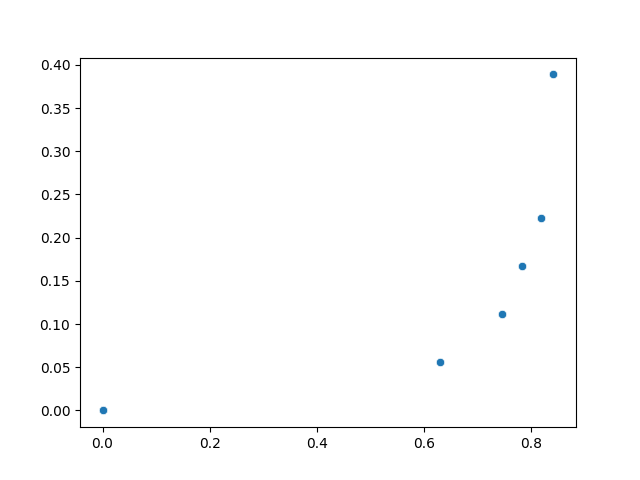
\includegraphics[width=\linewidth]{vehicle_94.png}
		\caption{Seed 94}
	\end{subfigure}
	\begin{subfigure}[b]{0.3\linewidth}
		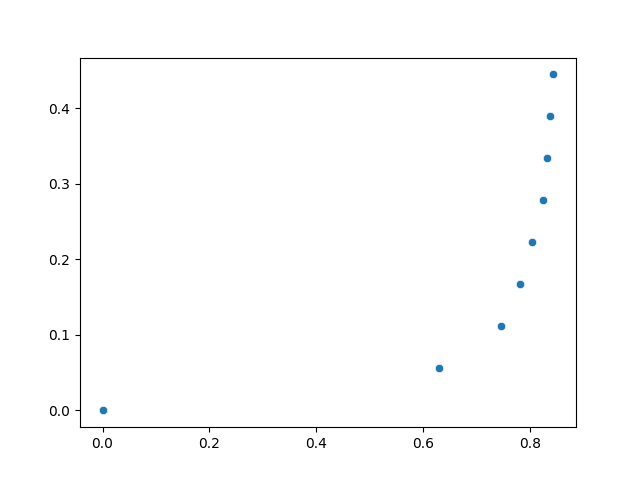
\includegraphics[width=\linewidth]{vehicle_102.png}
		\caption{Seed 102}
	\end{subfigure}
	\begin{subfigure}[b]{0.3\linewidth}
		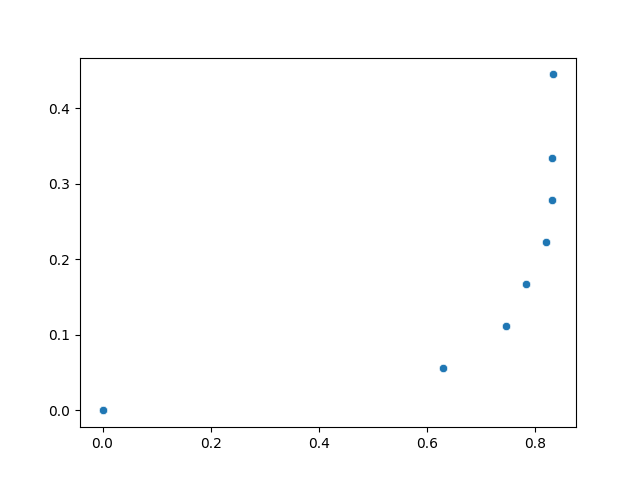
\includegraphics[width=\linewidth]{vehicle_151.png}
		\caption{Seed 151}
	\end{subfigure}
	\caption{Pareto front chart of vehicle dataset}
\end{figure}

\begin{figure}[h!]
	\centering
	\begin{subfigure}[b]{0.3\linewidth}
		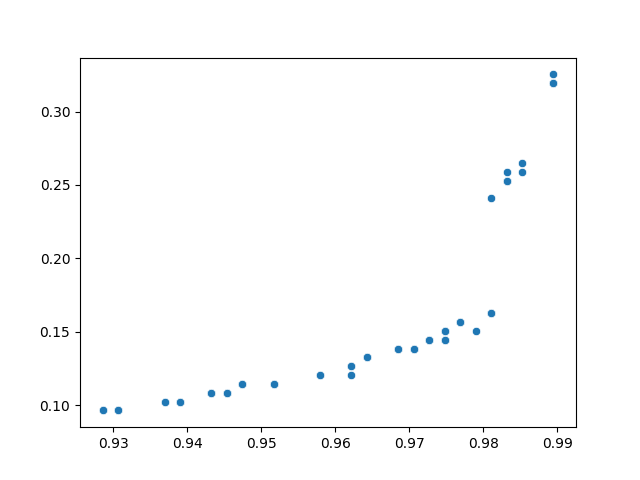
\includegraphics[width=\linewidth]{clean1_94.png}
		\caption{Seed 94}
	\end{subfigure}
	\begin{subfigure}[b]{0.3\linewidth}
		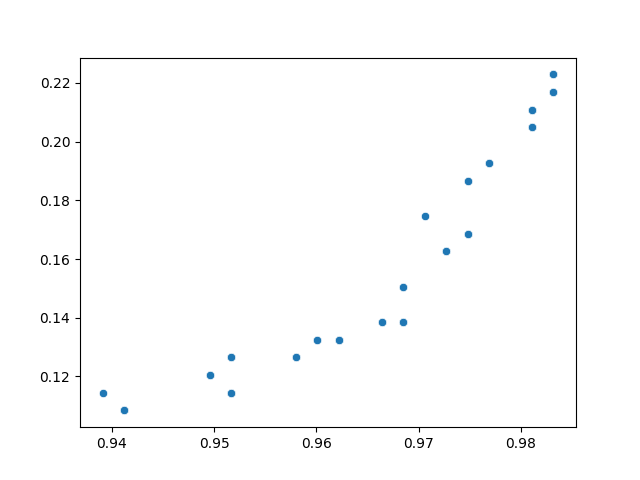
\includegraphics[width=\linewidth]{clean1_102.png}
		\caption{Seed 102}
	\end{subfigure}
	\begin{subfigure}[b]{0.3\linewidth}
		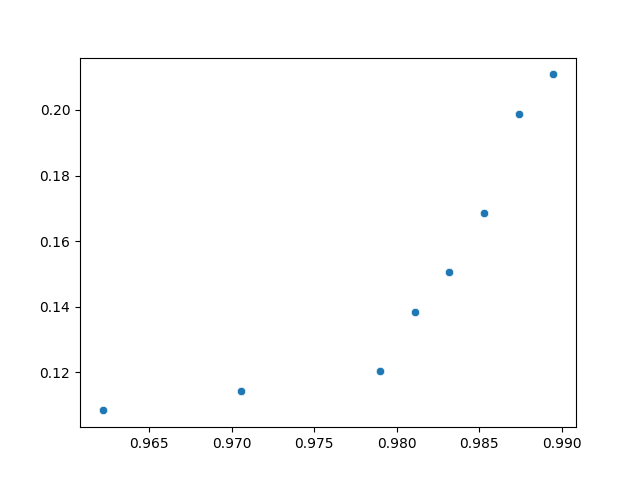
\includegraphics[width=\linewidth]{clean1_151.png}
		\caption{Seed 151}
	\end{subfigure}
	\caption{Pareto front chart of clean1 dataset}
\end{figure}
The vehicle dataset generated smooth Pareto fronts, indicating that it has converged for all seeds. This is expected because of the small number of features to select from. The clean1 dataset generated not as smooth fronts, indicating that because of the large number of features to select from, it still requires more generations to reach convergence. Even without achieving convergence the true Pareto front can be visually estimated from the generated points indicating that clean1 would achieve convergence with enough generations.
\subsection*{Conclusion}
NSGA2 can be used to determine a selection of features that has lower error rates compared to using all features, with NSGA2 achieving good results even before convergence. NSGA2 can still use the same genetic operators that GA uses with the difference being determining the elitism selection as NSGA2 and utilizing the domination relation and crowding distance in the fitness calculation. While NSGA2 works for 2 objectives, using more than 2 is not possible for this algorithm which limits the possible problems NSGA2 can be used for. 
\section*{Part 4}
\subsection*{Individual Representation}
Individuals are represented using a tree of functions and terminals. These trees are generated using the ramp-half-and-half method where half of the trees are generated using the grow method and the other half generated using the full method to encourage diversity in the population. The minimum and maximum height of the trees generated for the initial population is 1 and 4. 1 is chosen since having trees with smaller depth than 1 is not useful. 4 is chosen since at depth 4 a full tree will already have 31 nodes.
\subsection*{Function and Terminal Set}
For the function set, the arithmetic functions +, -(negation),* and \\(protected) are defined to allow the 1.0 constant to be any real number. The functions cos and sin are added since f(x) uses sin() and use of trig functions could improve the accuracy of the program. \par
\noindent For the terminal set, two constants are defined: x and 1.0. 1.0 is used to represent real number constants and can be transformed into any real number using the functions defined. X must be used since it is the parameter $f(x)$ uses.
\subsection*{Operators and Parameters}
For the genetic operators of GP: tournament selection, 1-point crossover and uniform mutation were chosen. Tournament selection was chosen because it provides a balance between exploration of the tree instance space and optimization. The tournament size was set to 5 to achieve the exploration/optimization balance as well. \par
\noindent 1-point crossover was chosen since swapping one subtree from each parent creates a unique enough child. \par 
\noindent Since there is no focus needed for creating more complicated trees or creating simpler trees, for mutation a uniform chance of mutating into a new subtree or just a terminal node is chosen. The possible subtrees generated in the mutation have sizes defined up to depth of 1, since having larger subtrees could make the trees too complicated and bloated too quickly. \par
\noindent To avoid very complicated trees which can be slow to evaluate and expensive in memory, the maximum depth for a tree was defined to be 17. 
\subsection*{Fitness}
For the fitness cases, the range defined for the x values needs to small enough such that the $f(x \leq 0)$ values are not so large that the GP ignores the variation generated by $sin(x)$ for the $f(x > 0)$ values. 30 x values evenly spread out in the range [-6.0, 15.0] were generated into the dataset to be used by the GP. More x values were defined at $x > 0$ to capture the $\frac{1}{x}$ effect on the $f(x > 0)$ values and to capture the $sin()$ pattern.\par
\begin{figure}[h!]
	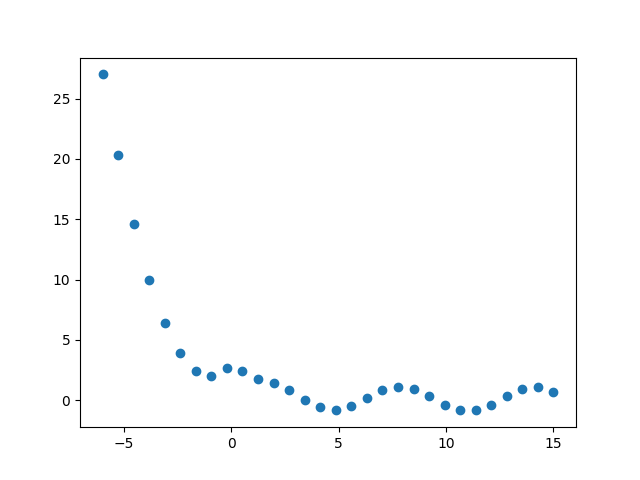
\includegraphics[width=\linewidth]{x_values.png}
	\caption{Range [-6.0,15.0] for x values used for fitness cases}
\end{figure}
\noindent For the fitness function, it is defined as the mean square error between the solution generated function and the problem defined function using the x values defined for the fitness cases. The aim of the GP is to minimize this mean square error value. \par
\subsection*{Discussion}
\begin{center}
\begin{tabular}{|c|c|}
\hline
Seed & MSE \\ 
\hline
94 & 2.946 \\
\hline
102 & 0.496 \\
\hline
151 & 0.368 \\
\hline
\end{tabular}
\end{center}

\begin{center}
\begin{tabular}{|c|c|}
\hline
Seed & Tree Depth \\
\hline
94 & 17 \\
\hline
102 & 16 \\
\hline
151 & 17 \\
\hline
\end{tabular}
\end{center}
For each seed, the best instance of the final generation is selected. Two of the three seeds generated trees that are at the maximum depth, indicating that the formulas generated are complicated. For the mean square error both seed 102 and 151 got $< 1.0$, seed 102 also has the smallest depth which shows that a higher depth does not lead to greater performance. \par
\begin{figure}[h!]
	\begin{subfigure}[b]{0.3\linewidth}
		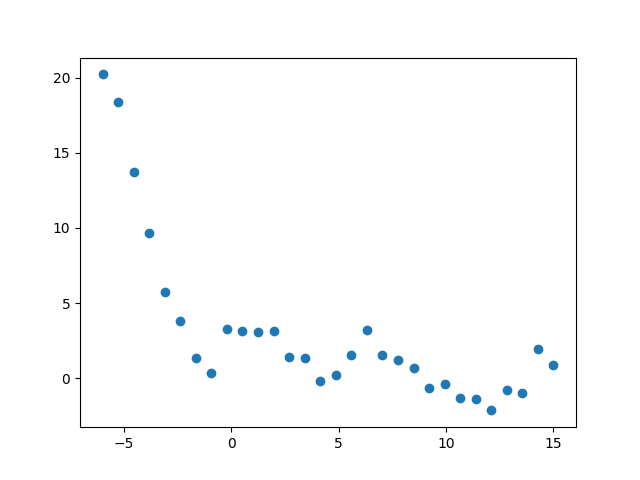
\includegraphics[width=\linewidth]{gp_94.png}
		\caption{Seed 94}
	\end{subfigure}
	\begin{subfigure}[b]{0.3\linewidth}
		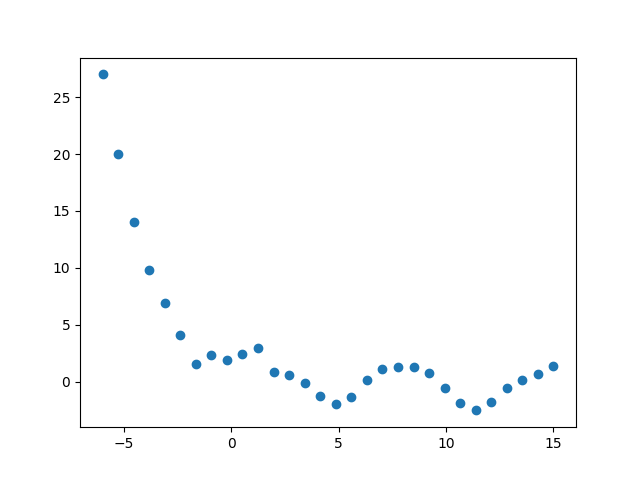
\includegraphics[width=\linewidth]{gp_102.png}
		\caption{Seed 102}
	\end{subfigure}
	\begin{subfigure}[b]{0.3\linewidth}
		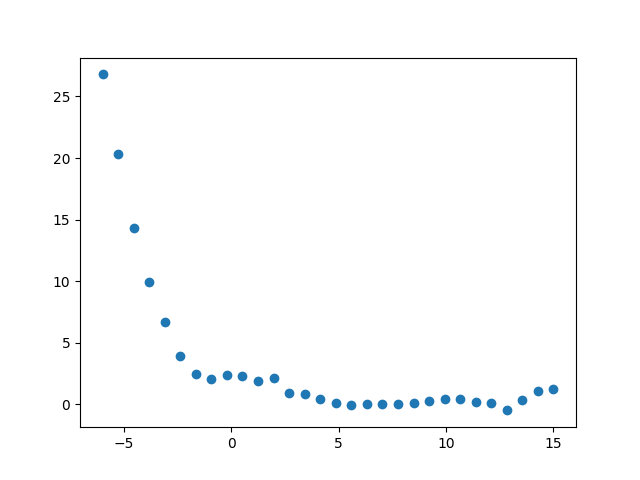
\includegraphics[width=\linewidth]{gp_151.png}
		\caption{Seed 151}
	\end{subfigure}
	\caption{Result values of GP generated functions}
\end{figure}
When looking at the result values generated by the best solution function, seed 94 has the least smooth function out of all the solution functions. Seed 151 does not capture the sin pattern present in the original function while seed 102 does. Though despite not capturing this pattern seed 151 has a lower mean square error, showing that the smoothness of the function is more important.  \par
\begin{figure}[h!]
	\centering
	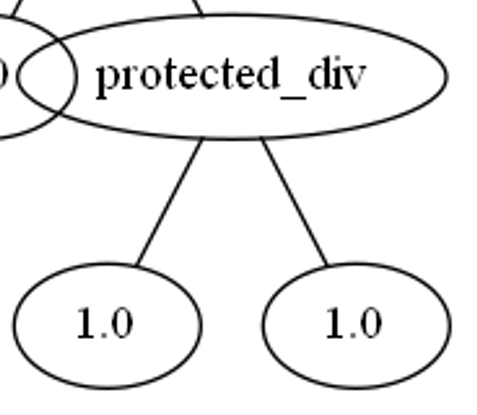
\includegraphics[width=0.5\linewidth]{redundant.png}
	\caption{Example of redundant calculations present in GP tree.}
\end{figure}
The trees often had redundant calculations being done, such as $\frac{x}{x}$ which can be simplified into terminal 1.0. When the number of generations increased, such cases became rarer. This happens because of the maximum depth constraint defined for the trees, where such cases need to be simplified into terminals to allow for more growth. Showing how defining such constraints prevents over complicated trees. \par
\begin{figure}[h!]
	\begin{subfigure}[b]{0.49\linewidth}
		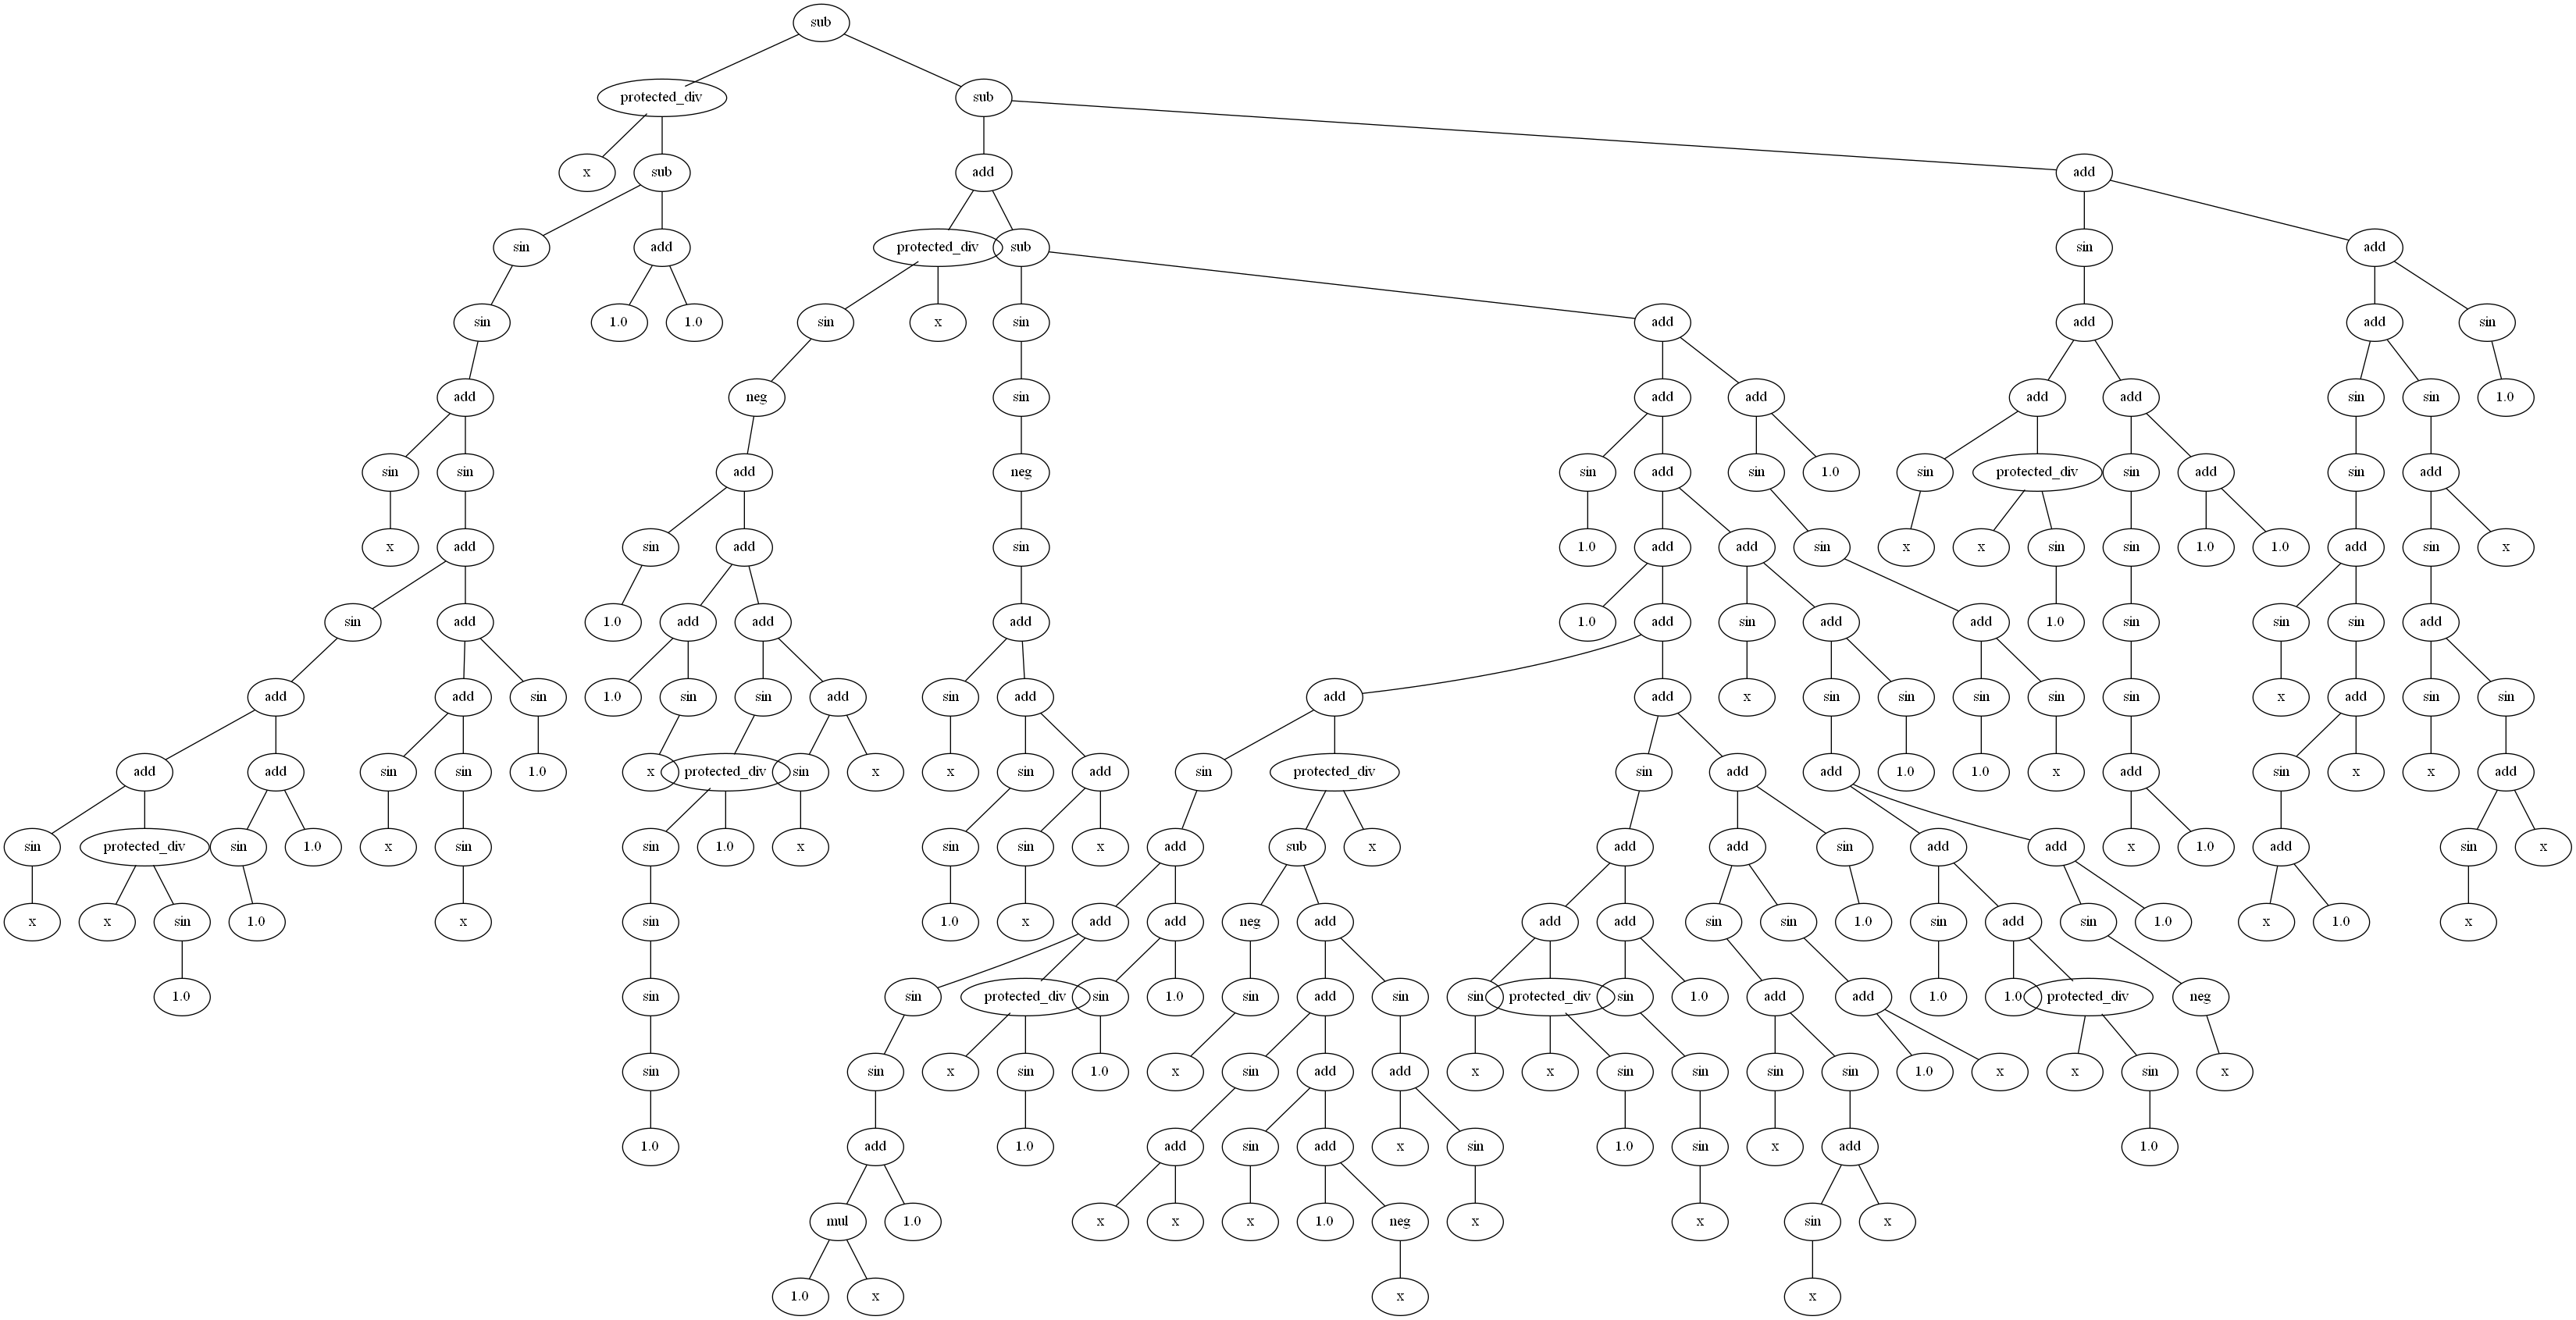
\includegraphics[width=\linewidth]{tree94.png}
		\caption{Seed 94}
	\end{subfigure}
	\begin{subfigure}[b]{0.49\linewidth}
		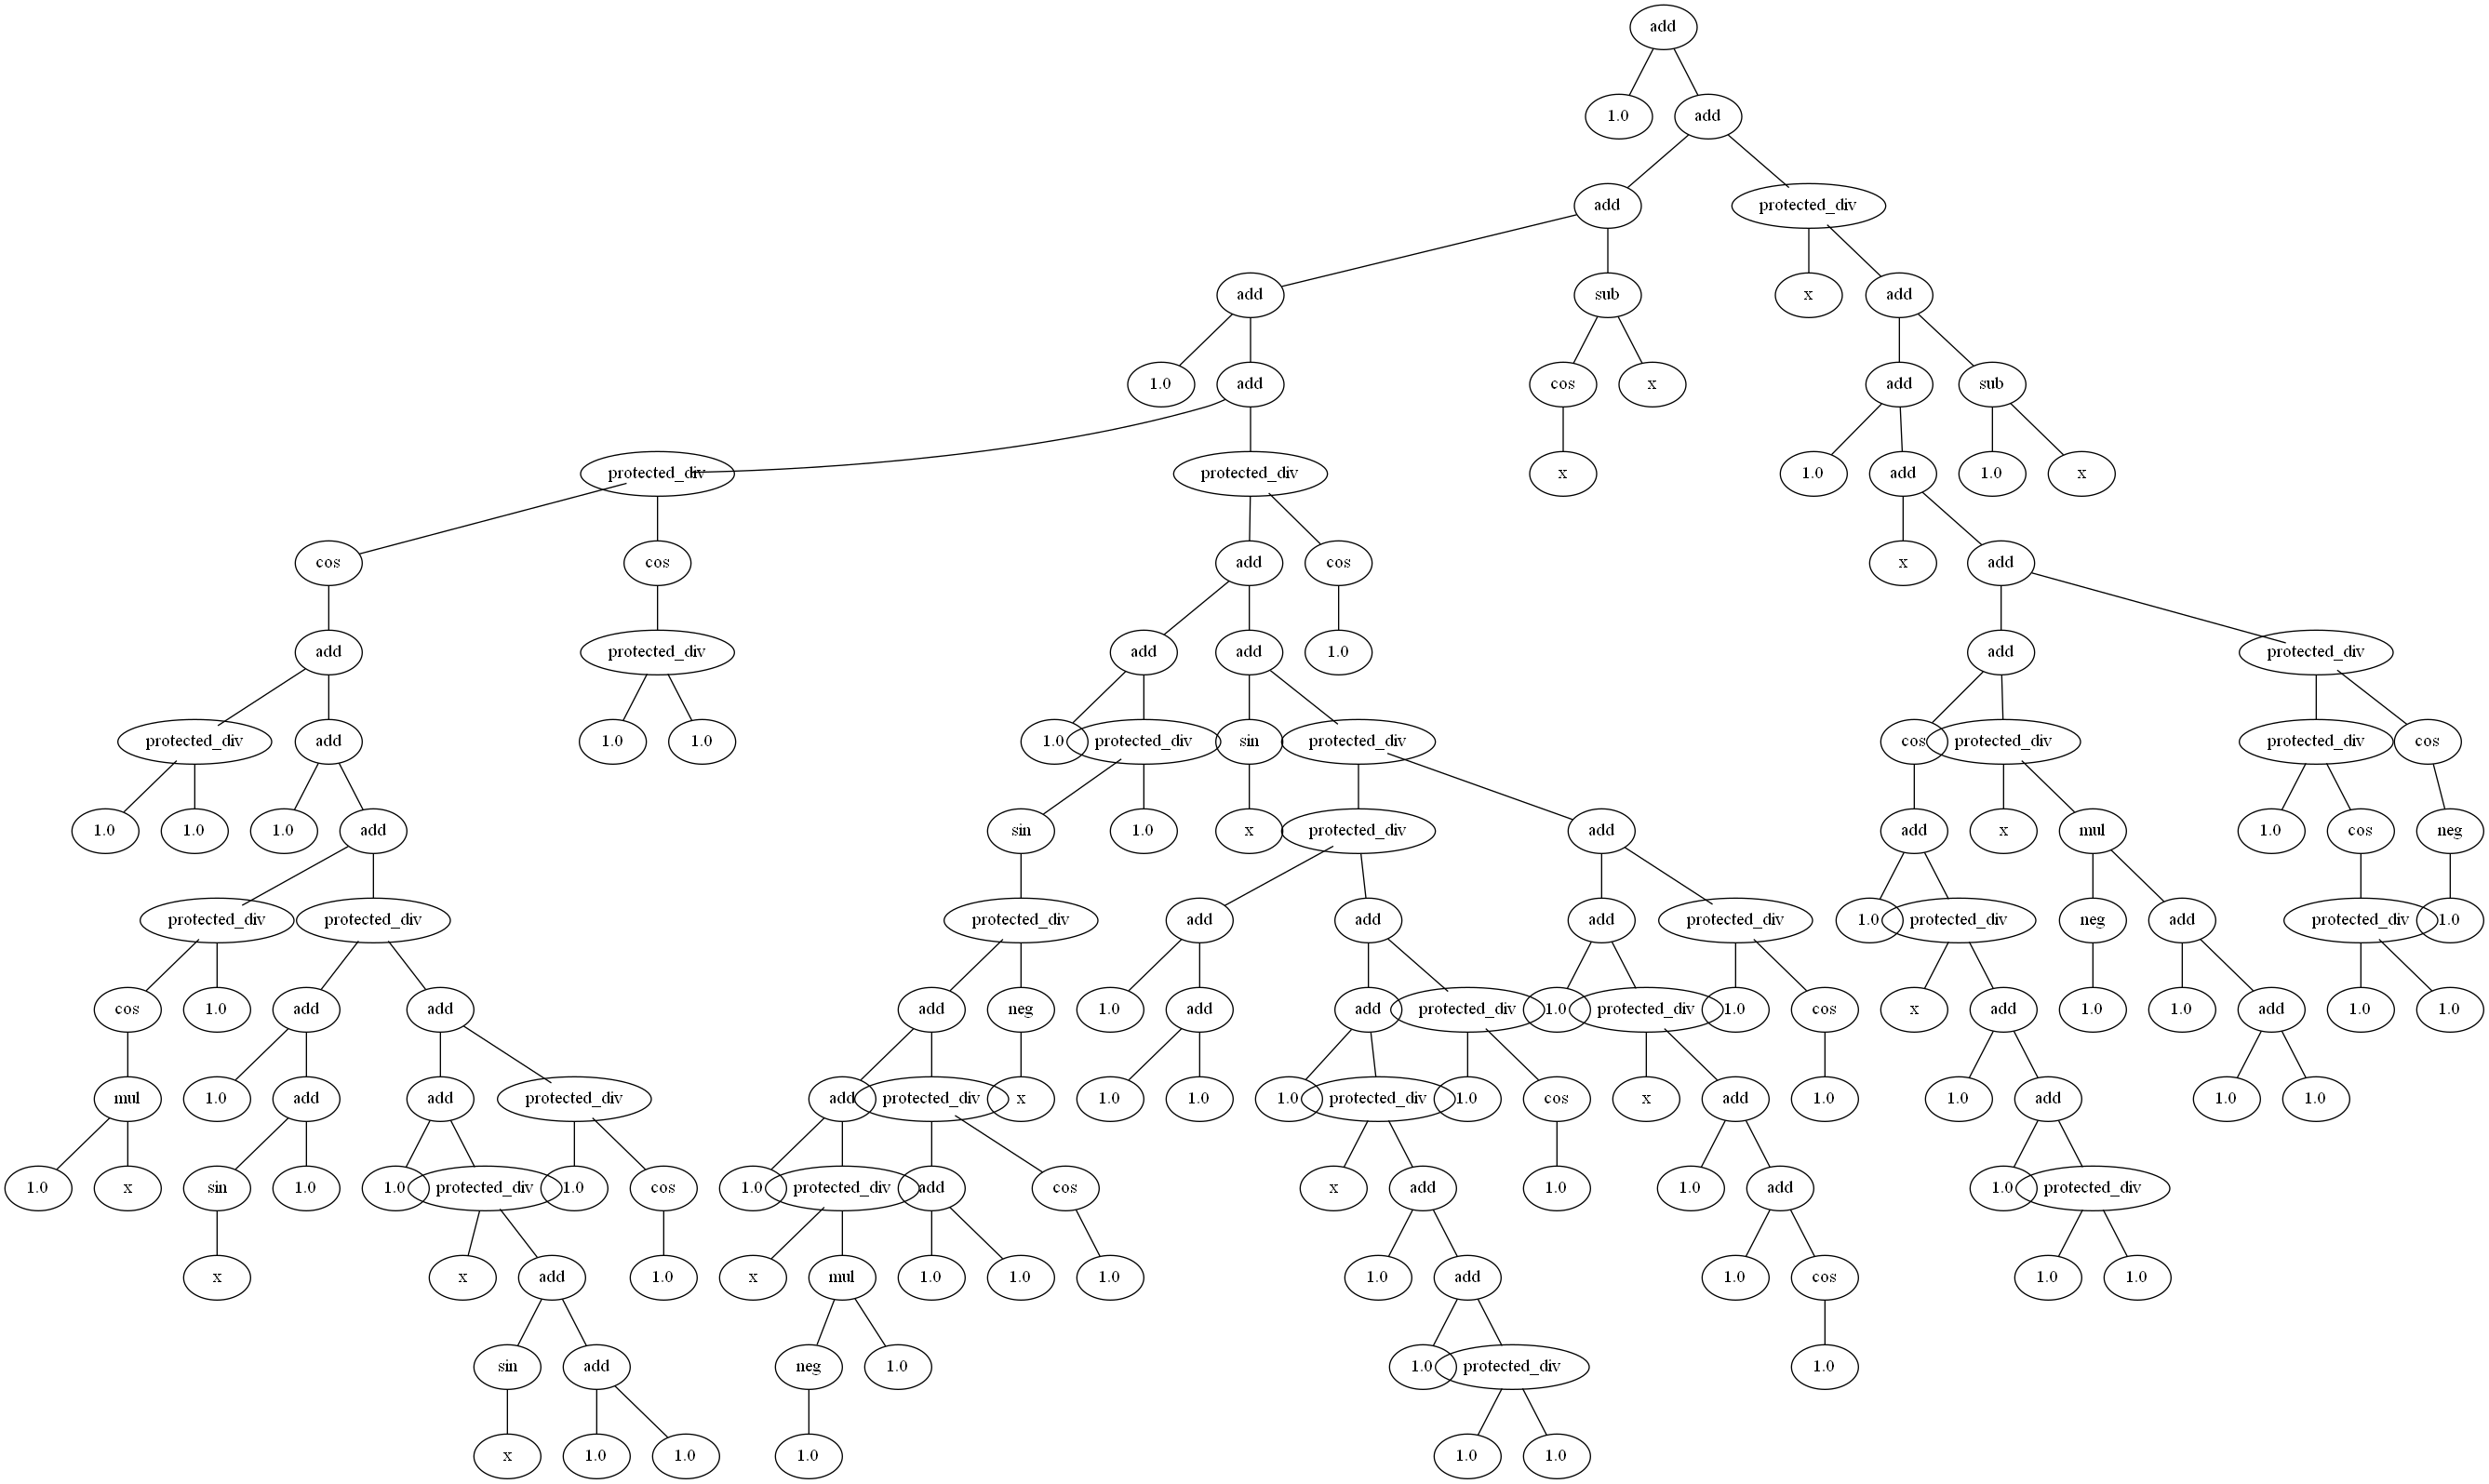
\includegraphics[width=\linewidth]{tree102.png}
		\caption{Seed 102}
	\end{subfigure}
	\begin{subfigure}[b]{0.49\linewidth}
		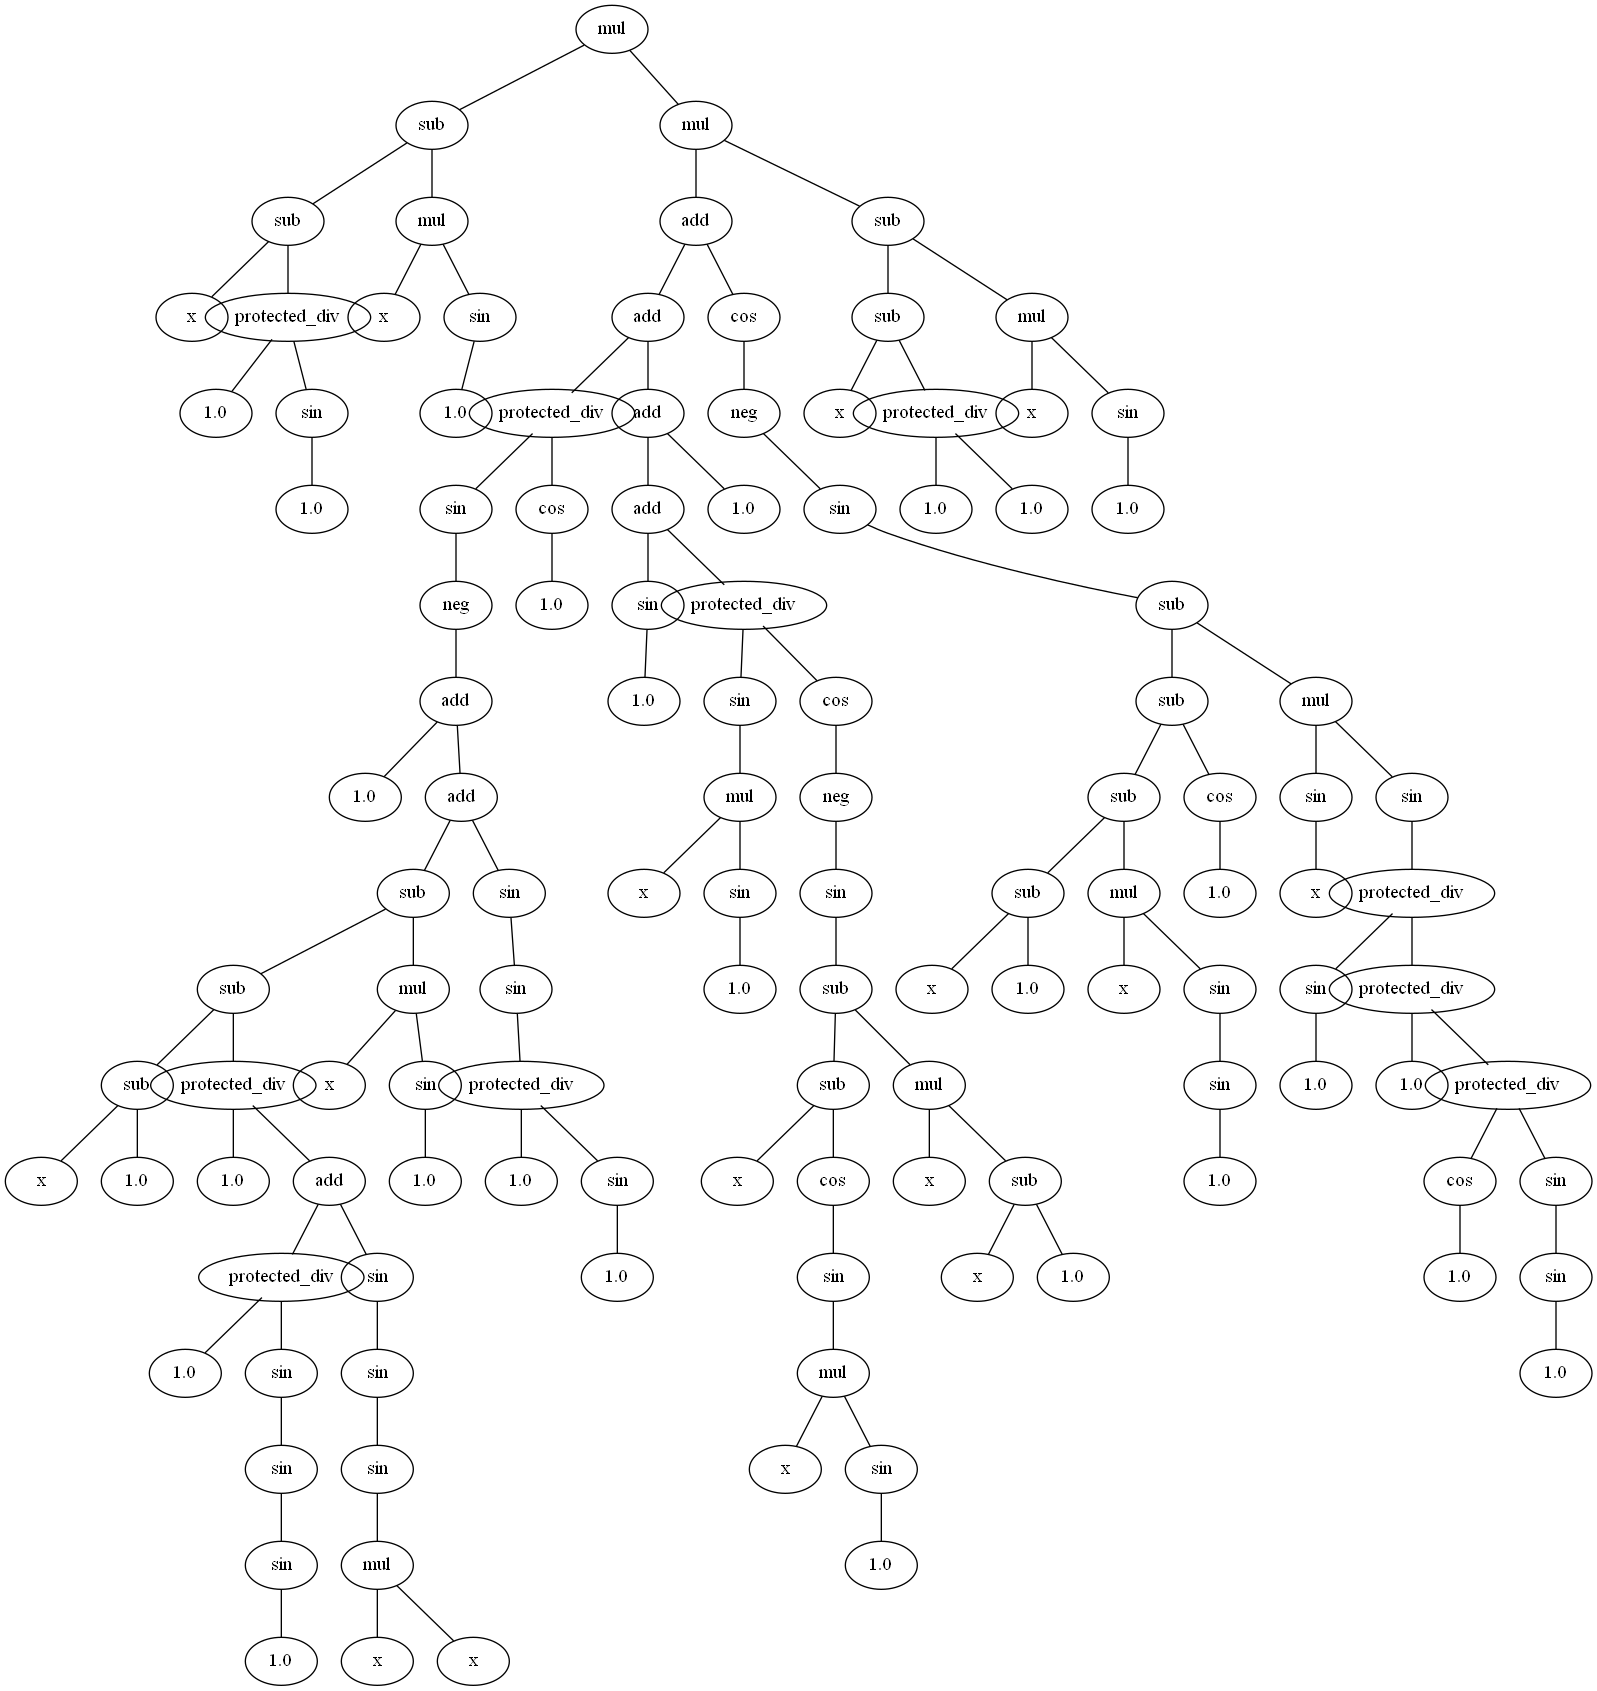
\includegraphics[width=\linewidth]{tree151.png}
		\caption{Seed 151}
	\end{subfigure}
	\caption{Resulting GP trees from seeds. Original images included in submission folder.}
\end{figure}
\subsection*{Conclusion}
It is possible to use GP to generate a function that mimics the values of the problem function without having to use conditional operators. This shows that GP is useful for recreating functions that mimic values of other functions that use different functions and terminals. With more iterations the GP will reach convergence where the generated function mimics the values of the problem function. For simplifying the function, stricter constraints on the depth of the trees or on the number of nodes allowed can be defined. But we will need to increase the number of generation and mutation rate to encourage exploration for the optimal solution. 
\section*{Part 5}
\subsection*{Particle Representation}
The space that the particles explore is the range of possible values for the variables used by the function. The particle’s position represents a possible combination of values for the variables and the particle’s velocity represents how much to change these values in the next generation. No encoding is needed for this particle representation since it stores the variables’ values directly. For the topology, since we are searching for the global minimum, the neighborhood for each particle is set to all other particles. \par
\subsection*{Parameters Used}
For the parameters used, since the Griewanks function has a lot of local minima present, exploration is encouraged to prevent the particles getting trapped in these local minima. So the inertia weight is increased to 1.1. For the Rosenbrock function where there is an easily identifiable global minima, exploitation is encouraged to reach the global minima sooner and thus is set to 0.8. Since the global minimum is likely found in the average personal and global best values, $\phi_1 = \phi_2$ is set with both values being set to 1.5. For the population size, the Rosenbrock function is more sensitive to the changes in the variables and thus needs a greater population size of 500 to find the minima compared to Griewanks’ function with a population size of 200. \par
\subsection*{Fitness}
For the fitness function, since the minimum value of the function is being determined, the output of the problem function with the instance variables' values is used for the fitness. The smaller the output, the greater the instance’s fitness becomes to encourage minimization. \par
\subsection*{Discussion}
\begin{center}
\begin{tabular}{|c|c|c|}
\hline
Problem Function & Mean & Standard Deviation \\
\hline
Rosenbrock D=20 & 68.418 & 75.158 \\
\hline
Griewanks D=20 & 0.148 & 0.0536 \\
\hline
Griewanks D=50 & 0.721 & 0.0784 \\
\hline
\end{tabular}
\end{center}
Rosenbrock's mean and standard deviation is much bigger than Griewanks' mean and standard deviation, this is because Rosenbrock has a much bigger output value range compared to Griewanks. \par 
\noindent When comparing the two Griewanks functions with $D = 20$ and $D = 50$, the former has a smaller mean and standard suggesting that $D = 20$ converges earlier than $D = 50$. Which is expected since $D = 50$ indicates that the particle swarm has to explore more dimensions to find the global minima. \par
\subsection*{Conclusion}
Particle swarm optimization for finding the global optima for problems where manual differentation can be difficult and/or very time consuming to achieve. While it does not give the exact solution for such problems, it is useful for situations where having a rough estimate of the answer is enough. \par
\noindent When comparing the result of searching for the global minima with different functions, the result needs to be standardized so that distribution of the function output values does not warp the comparison of fitness for different functions. \par
\end{document}